% !TeX root = Seminararbeit.tex

\documentclass[%
12pt,                % Schriftgröße
paper=a4,            % Papiergröße
captions=tableabove, % Beschriftungen für Tabellen oberhalb
]{scrartcl}

% ----------------------------------------------------
% Essential packages
% ----------------------------------------------------
\usepackage[utf8]{inputenc}
\usepackage[T1]{fontenc}

% ----------------------------------------------------
% Packages for layout adjustments
% ----------------------------------------------------

% Adjust line spacing
\usepackage{setspace}

% Publication quality tables
\usepackage{booktabs}

% ----------------------------------------------------
% Fonts
% ----------------------------------------------------
\usepackage{lmodern}
\renewcommand{\seriesdefault}{m}\selectfont

\newcommand\roboto{\fontfamily{Roboto-LF}\selectfont}
\newcommand*\robotocondensed{\roboto\fontseries{c}\selectfont}

\setkomafont{subject}{\large\robotocondensed}
\addtokomafont{title}{\LARGE}
\addtokomafont{subtitle}{\Large}
\setkomafont{author}{\normalsize\robotocondensed}
\addtokomafont{publishers}{\normalsize\robotocondensed}

% ----------------------------------------------------
% Colors
% ----------------------------------------------------
\usepackage{graphicx}
\usepackage[svgnames]{xcolor}
\definecolor{darkgreen}{rgb}{0.23,0.46,0.23}
\definecolor{smdsblue}{RGB}{0,69,134}

% ----------------------------------------------------
% Internal commands
% ----------------------------------------------------

\usepackage{etoolbox}
\makeatletter
\newcommand{\seminartype}[2]{%
  \subject{%
    Seminar\\
    \textit{\GetTranslationWarn{seminar@#1}}\\
    #2
  }
}
\newcommand{\advisor}[1]{%
  \publishers{%
    \GetTranslation{advisor}: #1\\
    \GetTranslation{institute}}
}
\newcommand{\email}[1]{\gdef\@email{#1}}
\newcommand{\matrno}[1]{\gdef\@matrno{#1}}
\newcommand{\institute}[1]{\gdef\@institute{#1}}
\newcommand{\useAI}[1]{\def\AIUse{#1}}
\makeatother

% Sprachauswahl:
%  main=* setzt die Hauptsprache für das Dokument
%  - ngerman --> deutsch
%  - english --> englisch
\def\languages{main=german,english}
%\def\languages{main=english,ngerman}

% Art und Zeitpunkt des Seminars:
% - SEvS    Software Engineering für verteilte Systeme
% - ML     Machine Learning
% - SEisS    Software Engineering in sicherheitskritischen Systemen
\seminartype{SEvS}{Sommersemester 2024}

% Haupttitel der Arbeit
\title{Recent Approaches to accelerate CP Solving}
% Untertitel der Arbeit -- für Seminararbeiten nicht benötigt
% \subtitle{Concepts, Technologies, and Applications}

% Name, Matrikelnummer und E-Mail-Adresse
\author{---}
\matrno{---}
\email{---e}

% Transparenzangabe zur Verwendung
% künstlicher Intelligenz (KI)-basierter Tools. 
% Mögliche Optionen:

% - No          Keine KI-basierten Tools verwendet:
%               Sämtliche Inhalte sind eigenständig und ohne die
%               Unterstützung von Algorithmen oder Software, 
%               die auf KI basiert, entstanden.

% - Support     Verwendung KI-basierter Tools zur sprachlichen 
%               Verbesserung oder Korrektur des Textes:
%               Dies umfasst die Nutzung von Software zur 
%               Grammatikprüfung, Rechtschreibkorrektur 
%               und stilistischen Optimierung des Textes. 

% - Content     Verwendung KI-basierter Tools zur (teilweisen) 
%               Generierung von Inhalt:
%               Dies beinhaltet die Nutzung von KI für die Erstellung 
%               von Textabschnitten, Konzeptionierung von Ideen oder
%               Bereitstellung struktureller oder inhaltlicher Vorschläge.

\useAI{Content}

% Datum der Abgabe
\date{---}

\advisor{---}

%%% Local Variables:
%%% mode: latex
%%% TeX-master: "Seminararbeit"
%%% End:


% ----------------------------------------------------
% Multi-lingual documents with Babel
% ----------------------------------------------------
\usepackage{csquotes}
\usepackage[\languages]{babel}

% ----------------------------------------------------
% Hyperlinks in PDF documents
% ----------------------------------------------------
\usepackage[%
bookmarks=true,         %
bookmarksopenlevel=1,   %
bookmarksopen=true,     %
bookmarksnumbered=true, %
plainpages=false,       % correct hyperlinks
pdfpagelabels=true,     % view TeX pagenumber in PDF reader
colorlinks=true,        % color highlight links
allcolors=black,        % make all links black by default
urlcolor=smdsblue,      % URL color
]{hyperref}

\makeatletter
\AtEndPreamble{
  \hypersetup{
    pdftitle=\@title,
    pdfauthor=\@author
  }
}
\makeatother

% Provides a solution to the problem with hyperref that links
% to floats actually anchor to the place below the float's caption,
% instead of anchoring to the beginning of the float
\usepackage[all]{hypcap}

% ----------------------------------------------------
% Code listings
% ----------------------------------------------------
\usepackage{listings}
\lstset{%
  frame=single,                             % Add a single line frame around listings
  frameround=ftft,                          % Rounded frame corners on top left and bottom right
  backgroundcolor=\color{gray!5},           % Slight gray shade for listings
  rulecolor=\color{black!30},               % Gray frame outline
  xleftmargin=.125\textwidth,               % Extra left margin
  xrightmargin=.125\textwidth,              % Extra right margin
  basicstyle=\small\ttfamily,               % General font style for listings
  keywordstyle=\bfseries,                   % Font style for keywords
  commentstyle=\color{gray},                % Font style for comments
  stringstyle={},                           % Font style for string literals
  numbers=left,                             % Show line numbers
  stepnumber=1,                             % Step increments for line numbers
  numberstyle={\sffamily\tiny\color{gray}}, % Font style for line numbers
  numbersep=2em,                            % Space between line numbers and code
}

% ----------------------------------------------------
% Bibliography management
% ----------------------------------------------------
\usepackage[%
backend=biber,      % Use biber to process bibliographies
natbib=true,        % Provide natbib-compatible citation commands
sorting=none,       % Sort citations by occurrence in the document
style=numeric-comp, % Use compressed numeric citations, e.g. [1-3; 5]
block=space,        % Add a little spacing inside bibliography entries
]{biblatex}
\addbibresource{literature.bib}

% Use main body font for URLs in bibliography
\urlstyle{same}

% Suppress page numbering on table of contents page(s). Works at least on one-page TOC.
\AtBeginDocument{\addtocontents{toc}{\protect\thispagestyle{empty}}} 

% Intelligent cross-referencing
% Note: Must be loaded at end of preamble (esp. after hyperref)
\usepackage{cleveref}

% ----------------------------------------------------
% Localization / translations
% ----------------------------------------------------
\usepackage{translations}

% Translations for seminar names
\NewTranslation{ngerman}{seminar@SEvS}{Software Engineering für verteilte Systeme}
\NewTranslationFallback{seminar@SEvS}{Software Engineering for Distributed Systems}
\NewTranslation{ngerman}{seminar@MS}{Machine Learning}
\NewTranslationFallback{seminar@MS}{Machine Learning}
\NewTranslation{ngerman}{seminar@SEisS}{Software Engineering in sicherheitskritischen Systemen}
\NewTranslationFallback{seminar@SEisS}{Software Engineering in Safety- and Security-Critical Systems}

% Generic translation used in template
\NewTranslation{ngerman}{advisor}{Betreuer}
\NewTranslation{ngerman}{matrno}{Matrikelnummer}
\NewTranslation{ngerman}{institute}{Softwaremethodik für verteilte Systeme (Prof. Bauer)\\Universität Augsburg}
\NewTranslation{ngerman}{regularlit}{Literatur}
\NewTranslation{ngerman}{onlinelit}{Online-Quellen}
\NewTranslation{ngerman}{honesty@title}{Eidesstattliche Erklärung}
\NewTranslation{ngerman}{honesty@body}{%
  Ich versichere, dass ich die vorliegende Arbeit ohne fremde Hilfe und ohne Benutzung anderer
  als der angegebenen Quellen angefertigt habe, und dass die Arbeit in gleicher oder ähnlicher
  Form noch keiner anderen Prüfungsbehörde vorgelegen hat.\endgraf
  Alle Ausführungen der Arbeit, die wörtlich oder sinngemäß übernommen wurden, sind als solche
  gekennzeichnet.
}
\NewTranslation{ngerman}{aiused@no}{%
  Bei der Erstellung dieses Dokuments wurde keinerlei auf künstliche Intelligenz 
  (KI)-basierte Software verwendet.
}
\NewTranslation{ngerman}{aiused@support}{%
  Bei der Erstellung dieses Dokuments wurde künstliche Intelligenz (KI)-basierte 
  Software ausschließlich zur sprachlichen Verbesserung und Korrektur verwendet. 
}
\NewTranslation{ngerman}{aiused@content}{%
  Bei der Erstellung dieses Dokuments wurde künstliche Intelligenz (KI)-basierte 
  Software zur Generierung von Inhalten verwendet. 
}


% English fallback text
\NewTranslationFallback{advisor}{Advisor}
\NewTranslationFallback{matrno}{Matriculation number}
\NewTranslationFallback{institute}{Software Methodologies for Distributed Systems (Prof. Bauer)\\University of Augsburg}
\NewTranslationFallback{regularlit}{Literature}
\NewTranslationFallback{onlinelit}{Online resources}
\NewTranslationFallback{honesty@title}{Declaration of Academic Honesty}
\NewTranslationFallback{honesty@body}{%
  Hereby, I declare that I have composed the presented paper independently on my own and without
  any other resources than the ones indicated. All thoughts taken directly or indirectly from external
  sources are properly denoted as such.\endgraf
  This paper has neither been previously submitted to another authority nor has it been published yet.
}
\NewTranslationFallback{aiused@no}{%
  No artificial intelligence (AI)-based software was used in the creation of this document.
}
\NewTranslationFallback{aiused@content}{%
  Artificial intelligence (AI)-based software was used for content generation in the 
  creation of this document.
}
\NewTranslationFallback{aiused@support}{%
Artificial intelligence (AI)-based software was used exclusively for linguistic improvement 
and correction in the creation of this document.
}


%%% Local Variables:
%%% mode: latex
%%% TeX-master: "Seminararbeit"
%%% End:


\begin{document}
\pagenumbering{roman}	
% !TeX root = Seminararbeit.tex

\begin{titlepage}
  \onehalfspacing
  \makeatletter
  \vspace*{1em}
  \begin{center}
    \ifdefempty{\@subject}{}{%
      {\usekomafont{subject}\@subject}
      \par\vspace{2em}
    }
    {\usekomafont{title}\@title}
    \ifdefempty{\@subtitle}{}{%
      \par\vspace{.5em}
      {\usekomafont{subtitle}\@subtitle}
    }
    \par\vspace{2em}
    \singlespacing
    {\usekomafont{author}%
      \@author\par
      \GetTranslation{matrno}: \@matrno\par}
    \texttt{\@email}
    \par\vspace{1.5em}
    {\usekomafont{publishers}\@publishers}
  \end{center}
  \makeatother

  \begin{abstract}
    \noindent%
    \paragraph*{\abstractname}
    \textcolor{red}{Bitte Dateien \texttt{settings.tex} und \texttt{titlepage.tex} anpassen.}
    
    Abstract Lorem ipsum dolor sit amet, consectetuer adipiscing elit, sed diam nonummy nibh euismod tincidunt ut laoreet dolore magna aliquam erat volutpat. Ut wisi enim ad minim veniam, quis nostrud exerci tation ullamcorper suscipit lobortis nisl ut aliquip ex ea commodo consequat.
  \end{abstract}

  \vfill
  \centering
  
\includegraphics[height=38mm]{figures/uni_siegel}
\end{titlepage}
%%% Local Variables:
%%% mode: latex
%%% TeX-master: "Seminararbeit"
%%% End:


\tableofcontents

\clearpage
\pagenumbering{arabic}


\section{Einleitung: Verwendung von Constraint Programming}
\label{sec:Einleitung-Verwendung-von-Constraint-Programming}

Constraint Programming (CP) spielt in vielen modernen Anwendungen eine große
Rolle, in denen Optimierungsprobleme mit Nebenbedingungen gelöst werden müssen.
Anwendungen hierzu sind unter anderem: Vehicle Routing, Scheduling, Planung,
Konfiguration, Ressourcenallokation und Kombinatorische Optimierung. Jedes Jahr
findet die Conference on Principles and Practice of Constraint Programming
statt, in der aktuelle Forschungsergebnisse im Bereich CP diskutiert werden, was
die Wichtigkeit des Themenfeldes unterstreicht \cite{CP20we}. Neben dem
klassischen Problem der Kursplanung \cite{duboi96jo} in einer sich ständig
beschleunigenden Zeit gibt es auch in der Industrie eine Vielzahl von
Scheduling-Problemen, wie die Zuweisung von Aufträgen zu Maschinen
\cite{gedik16jo}. Auch wurden CP-Ansätze für die Konfiguration von Netzwerken
verwendet \cite{ardisjo}. Ein weit verbreitetes kombinatorisches
Optimierungsproblem ist das 3-SAT-Problem, das beschreibt, ob eine Formel in
konjunktiver Normalform (KNF) mit Klauseln aus jeweils 3 Literalen erfüllbar ist
\cite[271]{rossi06bo}. 

Beispielsweise löst

\[ x_1=\text{false}, x_2=\text{false}, x_3=\text{false}, x_4=\text{false} \]

das folgende 3-SAT-Problem:

\[ (\lnot x_1 \lor x_2 \lor x_3) \land (x_1 \lor \lnot x_2 \lor x_4) \land (x_2
\lor x_3 \lor \lnot x_4) \]

Besonders Vehicle Routing ist in der heutigen Zeit für viele Unternehmen in der
Logistikbranche und dem flexiblen Transport von großer Bedeutung
\cite[1]{delec22jo}. Je nach Anwendungen und Problemstellung können
unterschiedliche Constraint Programming Ansätze verwendet werden. Es existieren
verschiedene Toolsets, um Constraint Programming-Probleme zu lösen. Für das
Vehicle Routing Problem, welches das Problem beschreibt, den kürzesten Gesamtweg
für \( n \) Fahrzeuge und \( m \) Orte zu finden \cite[222]{labor18jo}, kann
beispielsweise der IBM ILOG CP Optimizer verwendet werden \cite{IBMIwe}. Je nach
Problemstellung gibt es eine Vielzahl weiterer Toolsets \cite{Solviwea}.
OR-tools von Google ist eine weitere Möglichkeit zur Lösung von Constraint
Programming (CP), Linear Programming (LP), Integer Programming (IP) und Boolean
Satisfiability (SAT) Problemen \cite{ORToowe}. Geocode ist eine
Open-Source-Variante basierend auf C++ \cite{GECODwe}, und Chuffed ist eine
Variante, die "lazy clause generation" ausnutzt, um CP-Probleme schneller zu
lösen \cite{Chuff24co}. MiniZinc vereint unter anderem die zuvor beschriebenen
Softwarebibliotheken zu einer Ausdruckssprache zum Lösen einer Vielzahl von LP,
Transportproblemen (TP) und SAT-Problemen \cite{MiniZwe}. Unter demselben Namen
wird jährlich die MiniZinc Challenge ausgetragen, in der ein Parcours von
Constraint-Modellen gelöst werden muss. Am Ende werden die Solver nach Anzahl
der gelösten Modelle, der Zeit und der Qualität der Lösung bewertet
\cite{Homewe}. Gerade bei großen Problemstellungen, oder wenn, wie in der
Forschung oft üblich, mehrere Lösungen benötigt werden oder besondere Ansprüche
an die Qualität und Genauigkeit der Lösung gestellt werden, kann die Ausführung
oft lange dauern, weshalb die benötigte Zeit der Solver von großer Bedeutung
ist. Die folgende Arbeit soll aktuelle Ansätze vorstellen, mit denen CP-Probleme
schneller gelöst werden können.


\section{Grundlagen}
\label{sec:Grundlagen}
Grundsätzlich gibt es zwei Arten von Constraint-Problemen: Constraint
Satisfaction Probleme (CSP) und Constraint Optimization Probleme (COP). Ein CSP
beschreibt im Wesentlichen ein Problem, bei dem Nebenbedingungen festlegen,
welche Werte die Variablen annehmen können \cite[13]{rossi06bo}. Das Ziel
hierbei kann es entweder sein zu überprüfen, ob eine Lösung existiert, eine
mögliche Lösung zu finden oder die Menge aller möglichen Lösungen zu bestimmen.
Ein COP ist eine Erweiterung des CSP, bei dem zusätzlich eine Zielfunktion
minimiert werden muss \cite[171]{rossi06bo}. Ebenso kann es hierbei auch darum
gehen zu überprüfen, ob das Problem überhaupt lösbar ist, eine mögliche Lösung
zu finden oder die optimale Lösung zu finden.


\subsection{Constraint Satisfaction Probleme}
\label{sec:Constraint-Satisfaction-Probleme}

Ein CSP lässt sich durch ein Tripel \(P=(X,D,C)\) beschreiben, wobei \(X=\langle
x_{1},x_{2},\ldots,x_{n}\rangle\) ein n-Tupel von Variablen, \(D=\langle
D_{1},D_{2},\ldots,D_{n}\rangle\) ein n-Tupel von Domänen ist, so dass \(x_i\in
D_{i}\) erfüllt ist und \(C=\langle C_1,C_2,\ldots,C_t\rangle\) eine Menge von
Bedingungen beschreibt. Jede Bedingung \(C_j\) ist hierbei eine Untermenge des
kartesischen Produkts über \(D\). Eine Lösung für ein CSP ist ein n-Tupel
\(A=\langle a_1,a_2,\ldots,a_n\rangle \), so dass \(a_i\in D_i\) für alle \(i\)
und \(A \in C_j \quad \forall j\) \cite[16]{rossi06bo}. Ein Beispiel für ein CSP
ist das oben beschriebene 3-SAT-Problem. Das Lösen eines 3-SAT-Problems ist
NP-vollständig, was bedeutet, dass es keinen effizienten Algorithmus gibt, der
das Problem in Polynomialzeit lösen kann \cite[17]{rossi06bo}. Eine einfache
Möglichkeit, ein CSP zu lösen, ist die Verwendung von Backtracking. Hierbei wird
eine Variable nach der anderen belegt, und bei einem Widerspruch wird ein
Schritt zurückgegangen und eine andere Variable belegt \cite[21]{rossi06bo}.
Interessant ist auch, dass sich auch alle \(k>3\)-SAT-Probleme auf ein
3-SAT-Problem reduzieren lassen, wodurch auch das \(k>3\) SAT-Problem
NP-vollständig ist \cite[206]{gritz13bo}. Sind die Domänen der Variablen auf
boolesche Werte beschränkt, handelt es sich um ein Boolean Satisfiability
Problem (SAT).


\subsection{Constraint Optimization Probleme}
\label{sec:Constraint-Optimization-Probleme}

Viele Probleme in der realen Welt suchen nicht nur eine Lösung, sondern die
optimale Lösung. Solche Probleme lassen sich durch ein Constraint Optimization
Problem modellieren. Hierzu wird die Problemstellung um eine Zielfunktion
erweitert, die minimiert oder maximiert werden soll. Ein COP lässt sich durch
ein Tripel \(P=(X,D,C,f)\) beschreiben, wobei die ersten drei Elemente wie bei
einem CSP sind und \(f\) eine Zielfunktion ist \cite[22]{amadi15jo}. In der
Physik oder den Ingenieurwissenschaften werden COP oft auch in
Funktionsdarstellung beschrieben.

\[
\begin{aligned}
    &\text{minimiere:} \quad f(x) \\
    &\text{unter der Bedingung:} \\
    &\quad g_j(x) \leq 0 \\
    &\quad h_l(x) = 0 \\
    &\quad \underline{x_i} \leq x_i \leq \overline{x_i}
\end{aligned}
\]

Hierbei beschreiben \(g_j(x)\) und \(h_l(x)\) die Nebenbedingungen \(C\), wobei
erstere eine Ungleichungsrestriktion und letztere eine Gleichungsrestriktion
darstellt. Die letzte Gleichung beschreibt die Domäne \(D\) der Variablen
\cite[154]{marti21bo}. Je nach Art der Problemstellung unterscheiden sich die
verwendeten Algorithmen. Sind beispielsweise die Nebenbedingungen und die
Zielfunktion linear, handelt es sich um ein Linear Programming Problem (LP).
Dieses lässt sich beispielsweise mit dem Simplex-Algorithmus lösen. Das
Verfahren beruht darauf, dass die Nebenbedingungen einen n-dimensionalen
Polyeder aufspannen und die optimale Lösung auf einer Ecke des Polyeders liegt.
Der Simplex-Algorithmus sucht nun nacheinander die Ecken ab, bis die optimale
Lösung gefunden wurde. Beschränkt man sich bei den Lösungen auf ganzzahlige
Werte, spricht man von einem Integer Programming Problem (IP). Diese lassen sich
mit dem Branch-and-Bound-Algorithmus lösen \cite{dakin65jo}
\cite[99]{hofst07bo}.

\begin{figure}[h]
    \centering
    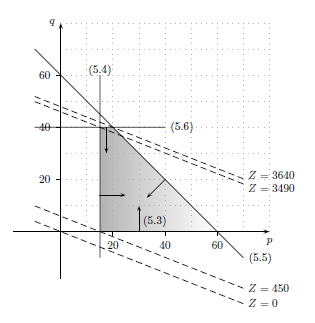
\includegraphics[width=0.5\textwidth]{figures/Simplex.PNG}
    \caption{Der Polyeder beschreibt die Nebenbedingungen, gestrichelte Linie
    die Zielfunktion, Ecken sind mögliche Lösungen \cite[100]{hofst07bo}}
    \label{fig:bild}
\end{figure}

Oft lassen sich Probleme jedoch nur über nichtlineare Zusammenhänge beschreiben.
Eine Möglichkeit, solche Probleme zu lösen, ist die Verwendung von
Gradientenverfahren \cite[153]{marti21bo}. Ein Problem bei der Verwendung dieser
ist jedoch, dass sie je nach Initialisierung oft nur lokale Minima finden
\cite[9]{boyd04bo}. Ein Ansatz, um dieses Problem zu umgehen, ist die Verwendung
von konvexen Funktionen. Dabei wird die nichtlineare Funktion durch eine konkave
Zielfunktion approximiert \cite[11]{boyd04bo}. Dies ist von Vorteil, da konvexe
Funktionen nur ein lokales Minimum haben \cite[7]{noced06bo}. Durch die
einfachere Lösbarkeit von konvexen Optimierungsproblemen spielen sie auch in der
Literatur eine wichtige Rolle \cite[8]{boyd04bo}.


\section{Recent Approaches To Accelerate Constraint Programs}
\label{sec:Recent-Approaches-To-Accelerate-Constraint-Programs}


\subsection{Portfolio Ansätze}
\label{sec:Portfolio-Ansätze}

Die Idee hinter Portfolio Ansätzen ist es, mehrere Solver zu kombinieren, um so
die Performance zu steigern. Es gibt verschiedene Ansätze, wie die Solver dabei
kombiniert werden können. Zum einen besteht die Möglichkeit, die Solver statisch
festzulegen, als auch dynamisch zu wählen. Weiter besteht die Möglichkeit des
Automatischen Parameter-Tunings, bei dem die Parameter der Solver automatisch an
das Problem angepasst werden \cite[8-11]{kotth12jo}. Eine weitere Fragestellung
ist die Wahl der Solver und wann dieser eingesetzt werden soll. Der am weitesten
verbreitete Ansatz ist, einen einzelnen Solver zu Beginn der Laufzeit zu wählen
und für das ganze Problem zu verwenden. Es gibt jedoch auch Ansätze, die den
Solver zur Laufzeit wechseln oder auch mehrere Solver aus dem Portfolio
gleichzeitig verwenden \cite[11-14]{kotth12jo}. Das Hauptproblem besteht jedoch
in der richtigen Wahl des Solvers. Während in den Anfängen die Algorithmen nach
handgewählten Kriterien ausgewählt wurden, werden heute oft automatische Ansätze
verwendet. Dazu zählen Lazy Approaches, wie das Abspeichern von Fallbeispielen
oder Nearest-Neighbor Ansätze. Auch wurden schon Klassifikationen,
Entscheidungsbäume, Support Vector Machines sowie Neuronale Netze verwendet.

\begin{figure}[h]
    \centering
    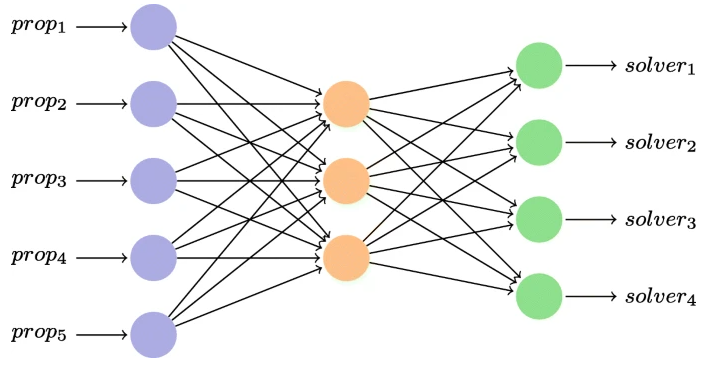
\includegraphics[width=0.5\textwidth]{figures/Neuronal Nework to choose Solver [popes22jo].PNG}
    \caption{Verwendung eines Neuronalen Netzes zur Wahl eines Solvers
    \cite[105]{popes22jo}}
    \label{fig:bild}
\end{figure}

Bei den Learning Ansätzen besteht jedoch das Problem, dass ein großer
Trainingsdatensatz benötigt wird \cite[15-16]{kotth12jo}. Eine weitere
Möglichkeit besteht darin, ein Performance-Modell der Solver zu lernen. Dadurch
kann einfach ein neuer Solver in das Portfolio aufgenommen werden, da die
Modelle für die bestehenden Solver nicht neu gelernt werden müssen
\cite[18]{kotth12jo}. Als Features für die Modelle können beispielsweise die
Anzahl der Variablen, die Anzahl der Constraints, die Domäne der Variablen oder
Verhältnisse der vorherigen Eigenschaften verwendet werden \cite[22]{kotth12jo}.
Ein Beispiel für einen Portfolio Solver ist der Sunny-Cp-Solver, welcher einen
lazy k-Nearest-Neighbor zur Auswahl eines Solver-Sets verwendet
\cite[4]{amadi15jo}.


\subsection{Model Based Optimization}
\label{sec:Model-Based-Optimization}

Sollte die objektive Funktion nicht bekannt sein und die Auswertung des
Blackbox-Modells teuer sein, kann Model Based Optimization verwendet werden, um
die Optimierung zu beschleunigen. Hierbei wird zunächst anhand einer kleinen
Anzahl von Auswertungen ein Modell der Blackbox erstellt, und dieses Modell wird
dann für die Optimierung verwendet. Auf diesem wird solange gearbeitet, bis ein
bestimmtes Budget, beispielsweise Schritte oder ein Delta-Wert, erreicht wird.
Mit diesem wird dann durch Auswertung der Blackbox das Ergebnis bestimmt,
welches entweder verwendet wird, um das Modell zu verfeinern, oder es wird als
Endresultat ausgegeben \cite[4]{bisch18pr}.


\subsection{Automated Parameter Tuning}
\label{sec:Automated-Parameter-Tuning}

Ein weiterer Ansatz, um die Performance von Solvern zu steigern, ist das
Automated Parameter Tuning. Hierbei werden die Parameter der Solver automatisch
an das Problem angepasst:

\[
\lambda^{*} \in \arg\max p(\mathcal{A}_{\lambda}, \mathcal{D})
\]

Hierbei beschreibt \(\lambda\) die Parameter des Algorithmus, \(\mathcal{A}\)
den Algorithmus und \(\mathcal{D}\) die Domäne. \(\lambda^{*}\) beschreibt die
optimalen Parameter für das Problem. Die Funktionsweise des Parameter Tunings
ist iterativ. Grundbaustein ist ein Konfigurator, welcher die Parameter des
Algorithmus anpasst. Initial werden dem Konfigurator die Parameter und die
Domäne übergeben. Der Konfigurator probiert verschiedene Konfigurationen aus und
übergibt sie dem Zielalgorithmus. Der Algorithmus wird auf das Problem
angewendet und gibt in Form einer Kostenfunktion an, wie gut die Konfiguration
war. Der Konfigurator passt iterativ auf Basis der Kostenfunktion die Parameter
an \cite[31-38]{kotth23pr}.

\begin{figure}[h]
    \centering
    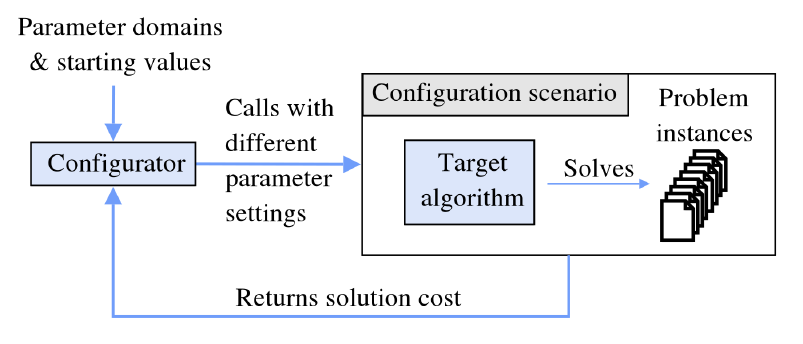
\includegraphics[width=0.5\textwidth]{figures/Automated Parameter Tuning [kotth23pr].PNG}
    \caption{Illustration des Parameter-Tuning-Prozesses \cite[34]{kotth23pr}}
    \label{fig:bild}
\end{figure}

Die Suche nach den optimalen Parametern kann entweder durch Grid Search oder
durch Random Search erfolgen. Bei der Grid Search werden die Parameter
systematisch abgedeckt. Bei der Random Search werden die Parameter zufällig
ausgewählt. Grid Search ist oft ineffizient, da eine große Anzahl von
unwichtigen Parameterkombinationen getestet werden. Dafür ist es aber
unwahrscheinlich, dass ein relevanter Bereich ausgelassen wird. Random Search
testet hingegen relevante Parameterkombinationen, jedoch auf zufällige Weise.
Dafür arbeitet Grid Search oft schneller, da mehr relevante
Parameterkombinationen getestet werden \cite[39]{kotth23pr}.

\begin{figure}[h]
    \centering
    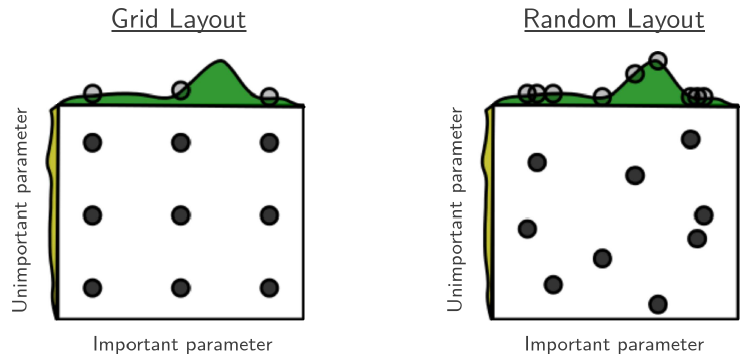
\includegraphics[width=0.5\textwidth]{figures/Grid Search vs. Random Search [kotth23pr].PNG}
    \caption{Grid Search und Random Search \cite[39]{kotth23pr}}
    \label{fig:bild}
\end{figure}

Ein weiterer Ansatz ist Local Search, bei dem ein einzelner Parameter iterativ
angepasst wird. Hierbei wird ein einzelner Parameter ausgewählt und verändert.
Falls die Veränderung zu einer Verbesserung führt, wird der Parameter behalten,
ansonsten verworfen.

%\subsection{Qunatum Acceleratedt} \label{sec:Qunatum Accelerated}

  
\subsection{Kombination von CP und SAT}
\label{sec:Kombination-von-CP-und-SAT}

Ein weiterer Ansatz, um CP-Probleme zu beschleunigen, ist die Kombination von CP
mit SAT. Hierzu wird die sogenannte Lazy Clause Generation verwendet. Diese
Methode wandelt die Constraints eines CP-Problems in SAT-Klauseln um. Diese
Klauseln werden nicht im Voraus generiert, sondern erst, wenn sie benötigt
werden. Durch die Verwendung von SAT Solvern können die Klauseln schneller
gelöst werden. Wenn es bei der Lösung eines SAT-Problems zu einem Konflikt
kommt, wird eine Klausel dem Solver hinzugefügt. Durch diese Kombination werden
die Stärken von CP (z. B. feinkörnige Domänenreduktion) und SAT (z. B.
leistungsstarke Konfliktlösung und Backtracking) optimal genutzt, was zu einem
effizienteren und leistungsfähigeren Solver führt \cite[5]{goosjo}. Ein Beispiel
für einen Solver, der diese Methode verwendet, ist der Chuffed Solver
\cite{Chuff24co}.


  
%\subsection{Decompostion methods} \label{sec:Decompostion methods}

  

\section{Schluss}
\label{sec:Schluss}
DDie vorgestellten Ansätze zur Beschleunigung von Constraint Programming (CP)
bieten vielfältige Möglichkeiten, die Leistungsfähigkeit von CP-Systemen zu
verbessern und damit die Lösung komplexer Probleme effizienter zu gestalten.

Portfolio-Ansätze zeigen, dass die Kombination mehrerer Solver eine
vielversprechende Strategie ist, um die Leistung zu steigern. Die dynamische
Auswahl oder die Kombination verschiedener Solver je nach Problemstellung kann
zu verbesserten Ergebnissen führen. Model Based Optimization und Automated
Parameter Tuning bieten weitere Wege, um die Effizienz von CP zu erhöhen, indem
Modelle verwendet oder Parameter automatisch angepasst werden.

Die Kombination von CP und SAT sowie die Nutzung von Lazy Clause Generation
stellen ebenfalls vielversprechende Ansätze dar, um die Leistung von CP-Systemen
zu steigern. Durch die Integration der Stärken beider Ansätze können komplexe
Probleme effizienter gelöst werden.

Es wird jedoch deutlich, dass es keinen universellen Ansatz gibt, um CP-Probleme
zu beschleunigen, da die Effektivität der Methoden stark von der spezifischen
Problemstellung abhängt. Vielmehr ist ein ganzheitlicher Ansatz erforderlich,
der die Auswahl und Kombination verschiedener Techniken je nach Problemstellung
und Ressourcen ermöglicht.

Die fortlaufende Forschung und Entwicklung auf diesem Gebiet verspricht, die
Leistungsfähigkeit von CP-Systemen weiter zu verbessern und ihre Anwendbarkeit
auf eine Vielzahl komplexer realer Probleme zu erweitern.

Es ist anzumerken, dass die vorgestellten Ansätze nur einen Teil des breiten
Spektrums der Forschung im Bereich der Beschleunigung von Constraint Programming
darstellen. Zukünftige Innovationen könnten auch durch neue Technologien wie
Quantum Computing beeinflusst werden.

Insgesamt bleibt die Optimierung von CP-Systemen ein aktives und vielschichtiges
Forschungsfeld, das weiterhin großes Potenzial für Innovationen und Fortschritte
bietet.


% Literaturverzeichnis
\printbibliography[heading=bibintoc]

% Anhang
\include{appendix}

% Eidesstattliche Erklärung
% !TEX root = Seminararbeit.tex

\clearpage
\section*{\GetTranslation{honesty@title}}
\GetTranslation{honesty@body}

\vspace{2em}

\ifdefined\AIUse
    \expandafter\ifstrequal\expandafter{\AIUse}{No}{%
        \GetTranslation{aiused@no}
    }{%
        \expandafter\ifstrequal\expandafter{\AIUse}{Content}{%
            \GetTranslation{aiused@content}
        }{%
            \expandafter\ifstrequal\expandafter{\AIUse}{Support}{%
                \GetTranslation{aiused@support}
            }{% Fallback for undefined values
                \GetTranslation{aiused@no}
            }%
        }%
    }%
\else
    % Fallback, falls \useAI{} nie aufgerufen wurde
    \GetTranslation{aiused@no}
\fi

\vspace{2em}
\makeatletter
Augsburg, \@date
\par\vspace{1.5cm}
(\@author)
\makeatother

%%% Local Variables:
%%% mode: latex
%%% TeX-master: "Seminararbeit"
%%% End:


\end{document}